\documentclass[10pt,a4paper]{article}
\usepackage[margin=0.7in]{geometry}
\usepackage{amsmath,amssymb}
\usepackage{array}
\usepackage{booktabs}
\usepackage{fancyhdr}
\usepackage{tikz}
\usetikzlibrary{positioning,shapes,arrows}

\pagestyle{fancy}
\fancyhf{}
\renewcommand{\headrulewidth}{0pt}

\begin{document}

\begin{center}
\begin{tabular}{|c|c|c|c|c|c|c|c|c|c|}
\hline
\multicolumn{10}{|c|}{USN} \\
\hline
& & & & & & & & & \\
\hline
\end{tabular}

\vspace{0.3cm}

{\Large \textbf{NMAM INSTITUTE OF TECHNOLOGY, NITTE}}\\[0.15cm]
{\small \textit{(An Autonomous Institution affiliated to VTU, Belagavi)}}\\[0.2cm]
{\large \textbf{IV Sem B.E. (CS/IS/AM/CC) Mid Semester Examinations -- II, June 2022}}\\[0.15cm]
{\large \textbf{20CS402 / 20IS402 /20AM402 / 20CC402 -- DESIGN AND ANALYSIS OF ALGORITHMS}}\\[0.2cm]
\end{center}

\noindent
\begin{tabular}{p{8cm}r}
\textbf{Duration:} 1 Hour & \textbf{Max. Marks:} 20
\end{tabular}

\vspace{0.15cm}
\begin{center}
\textit{Note: Answer any \textbf{One} full question from \textbf{each Unit}.}
\end{center}

\vspace{0.15cm}

\begin{center}
{\large \textbf{Unit -- I}}
\end{center}

\noindent
\begin{tabular}{|p{10.5cm}|c|c|c|c|}
\hline
\textbf{Question} & \textbf{Marks} & \textbf{BT*} & \textbf{CO*} & \textbf{PO*} \\
\hline
\textbf{1. a)} Develop an algorithm to perform Insertion Sort and analyze the best and worst case efficiencies. & 4 & L*4 & 3 & 2 \\
\hline
\textbf{b)} Find the solution for following problem using topological sorting method. Consider a set of 5 courses\{C1,C2,C3,C4,C5\}, a part time student has to take in some degree program. The courses can be taken in any order as long as the following course prerequisites are met: C1 and C2 have no prerequisites, C3 requires C1 and C2, C4 requires C3 and C5 requires C3 and C4. The student can take only one course per term. & 3 & L3 & 3 & 2 \\
\hline
\textbf{c)} Construct 2-3 tree for the data C,O,M,P,U,T,I,N,G. & 3 & L3 & 3 & 2 \\
\hline
\textbf{2. a)} Explain Horspool's algorithm and apply the algorithm to find the pattern ``MONEY'' in the text ``A FOOL AND HIS MONEY ARE PARTED SOON''. & 4 & L3 & 3 & 2 \\
\hline
\textbf{b)} Apply closed hashing to distribute the keys 10,23,14,19,17,32,45 using the function H(k) = K(mod11). & 2 & L3 & 3 & 2 \\
\hline
\textbf{c)} Construct heap and sort using array representation 2,9,8,14,22,16,7 & 4 & L3 & 3 & 2 \\
\hline
\end{tabular}

\vspace{0.3cm}

\begin{center}
{\large \textbf{Unit -- II}}
\end{center}

\noindent
\begin{tabular}{|p{10.5cm}|c|c|c|c|}
\hline
\textbf{Question} & \textbf{Marks} & \textbf{BT*} & \textbf{CO*} & \textbf{PO*} \\
\hline
\textbf{3. a)} Outline the pseudocode for Prims algorithm to find the minimum spanning tree. Apply the Prims algorithm to find the minimum spanning tree for the following graph

\begin{center}
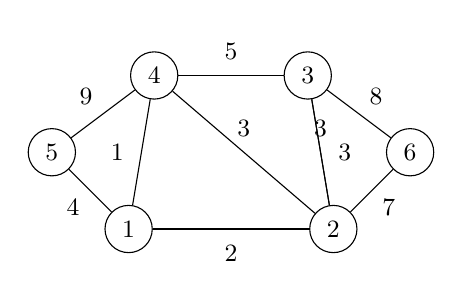
\begin{tikzpicture}[scale=0.65, every node/.style={circle, draw, fill=white, minimum size=6mm, inner sep=1pt, font=\small}]
\node (5) at (0,0) {5};
\node (4) at (2,1.5) {4};
\node (3) at (5,1.5) {3};
\node (6) at (7,0) {6};
\node (1) at (1.5,-1.5) {1};
\node (2) at (5.5,-1.5) {2};

\draw (5) -- node[above left, draw=none, fill=none] {9} (4);
\draw (4) -- node[above, draw=none, fill=none] {5} (3);
\draw (3) -- node[above right, draw=none, fill=none] {8} (6);
\draw (5) -- node[below left, draw=none, fill=none] {4} (1);
\draw (1) -- node[below, draw=none, fill=none] {2} (2);
\draw (2) -- node[below right, draw=none, fill=none] {7} (6);
\draw (4) -- node[left, draw=none, fill=none] {1} (1);
\draw (3) -- node[right, draw=none, fill=none] {3} (2);
\draw (3) -- node[above, draw=none, fill=none] {3} (2);
\draw (4) -- node[above, draw=none, fill=none] {3} (2);
\end{tikzpicture}
\end{center} & 6 & L3 & 4 & 2 \\
\hline
\textbf{b)} Write a pseudocode for Bellman Ford algorithm to find the single source shortest path. & 4 & L2 & 4 & 1 \\
\hline
\textbf{4. a)} Construct a Huffman code for the following data: \newline
\begin{tabular}{|c|c|c|c|c|c|}
\hline
Character & A & B & C & D & -- \\
\hline
Probability & 0.4 & 0.1 & 0.2 & 0.15 & 0.15 \\
\hline
\end{tabular} \newline
Encode the text ABACABAD using the code of obtained. Decode the text whose encoding is 100010111001010 & 6 & L3 & 4 & 1 \\
\hline
\textbf{b)} Write the pseudocode for single source shortest path in DAG. & 4 & L2 & ~ & ~ \\
\hline
\end{tabular}

\vspace{0.3cm}
\begin{center}
\small{BT* Bloom's Taxonomy, L* Level; CO* Course Outcome; PO* Program Outcome}\\[0.2cm]
******************
\end{center}

\end{document}
